\chapter{Modeling and Simulation}\label{c-ModSim}

Some systems cannot be practically tested.  Consider the spread of a highly infectious disease, or the destruction due to a nuclear war.  We can look at smaller examples of these, but the full blown case would be bad to run.  What we would like to do is to take our mathematical knowledge and create a system of equations which will have the same behavior.  We can then test the real system by seeing how the modeled system behaves.  This action of making a a mathematical model be similar to the real system is simulation (same root as similar).  Often these systems are expressed as either differential or difference equations.  They can thus be solved by our differential equation solvers directly, or transformed (Laplace, Fourier, Z, etc.) so they can be solved by zero-finding.

Lets look at how we can set some of these up, and then give some examples.

\subsection{Electric Circuit}
Kirkoff's law tells us that the sum of the voltage drops around a loop must be zero.  We can use this to figure out how to set up some models.  To do so we need to note how each element operates.  On the attached sheets I have included some copies of physical elements and how they relate.  If we consider our basic variable as charge then current is just the time derivative of charge and we can see the elements are just:
\beqn
V_{inductor} & = & L\ddot{q} \\
V_{resistor} & = & R\dot{q} \\
V_{capacitor} & = & \frac{1}{C}q
\eeqn
We can then write an equation for each loop and plot the first derivative of each of the loop charges (thus loop current).

\subsubsection{Low Pass Filter}

The sums of the voltage drops around the loop is
\begin{eqnarray}
V_{in} - R\dot q -\frac{1}{C}q &=& 0\label{eq-diffeqmodel-lowpassfilter}
\end{eqnarray}
The output voltage is the voltage across the capacitor, so
\begin{eqnarray}
V_{out} &=&\frac{1}{C}q
\end{eqnarray}
We thus need to find $q$, and we know (rearranging eq~\ref{eq-diffeqmodel-lowpassfilter})
\begin{eqnarray}
\dot q &=& \frac{V_{in}}{R} -\frac{1}{RC}q
\end{eqnarray}
This equation becomes code~\ref{code:lowpass}.
\SciLab{Code for the differential equation describing a low pass filter.}{code:lowpass}{scilab/lowpass.sci}
When called by
\SciLab{Code to simulate a low pass filter using RK 2nd order.}{code:lowpassfilter}{scilab/lowpassfilter.sce}

\begin{figure}
\begin{center}
\caption{Input and output voltages of the low pass filter.}
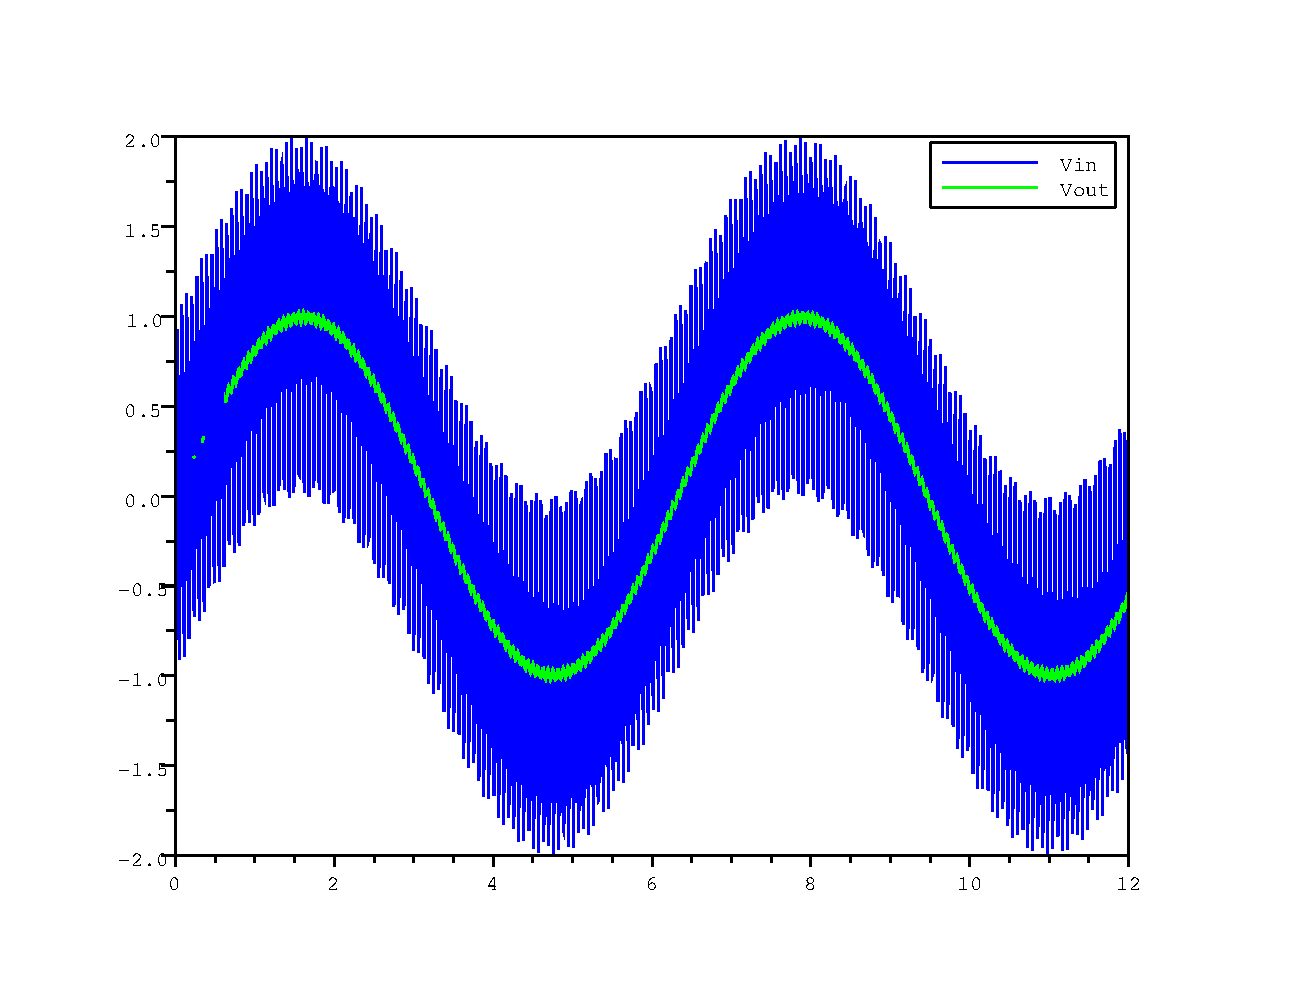
\includegraphics[width=.8\textwidth]{lowpass}
\end{center}
\end{figure}

\subsection{System of Masses}
Consider a system of masses connected by springs and dampers.  We can note that the if we choose our variable to be position then we have:
\beqn
F_{spring} & = & -kx \\
F_{damper} & = & -c\dot{x} \\
F_{mass} & = & m\ddot{x}
\eeqn

\subsection{Linearized Pendulum}
\beqn
\dot{\left[\begin{matrix}x_{1}\cr
                   x_{2}\end{matrix}\right]}
=
\left[\begin{matrix}0 & 1\cr
              -\sqrt{\frac{g}{l}}  & -c\end{matrix}\right]
\left[\begin{matrix}x_{1}\cr
              x_{2}\end{matrix}\right]
\eeqn


\subsection{Fox and Rabbits}

Consider the problem where there is a predator and its prey in the area.  If there are too many predators they might eat off all the prey and starve themselves.  If there are too much of the prey the predators will increase in number because of the plentiful food.  How do we model this?

We want several things in our model. First, predators should naturally starve, only the presence of prey offsets this.  Prey should naturally breed, and predators offset this.  The offset to both should be a scaled proportion of the contacts.  Contact should be rare when either population is low and more frequent with a reasonable number of both.  These considerations lead to the model that contacts occur at a rate proportional to the product of predators and prey.  These rules are combined in the model below.

\beqn
\dot{\bmat x_{1}\cr
           x_{2}\emat}
&=&
\bmat -m_{1} & 0\cr
       0     & m_{2}\emat
\bmat x_{1}\cr
      x_{2}\emat+
\bmat  b_{1}x_{1}x_{2}\cr
      -b_{2}x_{1}x_{2}\emat \\
&=&
\bmat b_{1}x_{2}-m_{1} & 0\cr
      0                & m_{2}-b_{2}x_{1}\emat
\bmat x_{1}\cr
      x_{2}\emat
\eeqn

To keep the population constant in each we need $b_{1}x_{2}-m_{1}=0$ and $m_{2}-b_{2}x_{1}=0$, thus
\beqn
x(1)&=&\frac{m_2}{b_2} \\
x(2)&=&\frac{m_1}{b_1}
\eeqn

We can implement the basic predator prey rate calculations by the Scilab function
\begin{verbatim}
function [xdot]=predator_prey_rate(starve,birth,eat,eaten,predator,prey)
    xdot=zeros(2,1);
    xdot(1)=(eat*prey-starve)*predator;
    xdot(2)=(birth-eaten*predator)*prey;
endfunction
\end{verbatim}
To specialize this to our foxes and rabbits we could write the Scilab function
\begin{verbatim}
function [xdot]=fox_rabbit(t,x)
    starve=5;
    birth=10;
    eat=.01;
    eaten=.5;
    predator=x(1);
    prey=x(2);
    getf('predator_prey_rate.sce');
    xdot=predator_prey_rate(starve,birth,eat,eaten,predator,prey);
endfunction
\end{verbatim}
Now we need to solve it, so we will use the function ode.  The following code will set everything up for us and call ode.
\begin{verbatim}
getf('fox_rabbit.sce');
x=ode([22;500],0,[0:.01:10],fox_rabbit);

//set("figure_style","new") //create a figure
subplot(211)
   plot2d([0:.01:10],x')
   xtitle('Fox and Rabbit History','Years','Population');
subplot(212)
   plot2d(x(1,:),x(2,:))
   xtitle('Fox and Rabbit Interaction','Foxes','Rabbits');
\end{verbatim}
When we run it we get the following graphic.
\begin{figure}[h]
\begin{center}
\leavevmode
\hbox{
\epsfxsize=6in
\epsffile{foxesNrabbits2.eps}}
\end{center}
\caption{Foxes and Rabbits}
\label{f-foxrabbit}
\end{figure}


\subsection{Arms race}
\beqn
\dot{\left[\begin{matrix}x_{1}\cr
                   x_{2}\end{matrix}\right]}
=
\left[\begin{matrix}-m_{1} & a_{1}\cr
              a_{2}  & -m_{2}\end{matrix}\right]
\left[\begin{matrix}x_{1}\cr
              x_{2}\end{matrix}\right] +
\left[\begin{matrix}b_{1}x_{2}^{2}\cr
              b_{2}x_{1}^{2}\end{matrix}\right]
\eeqn
